\begin{sidewaysfigure}
  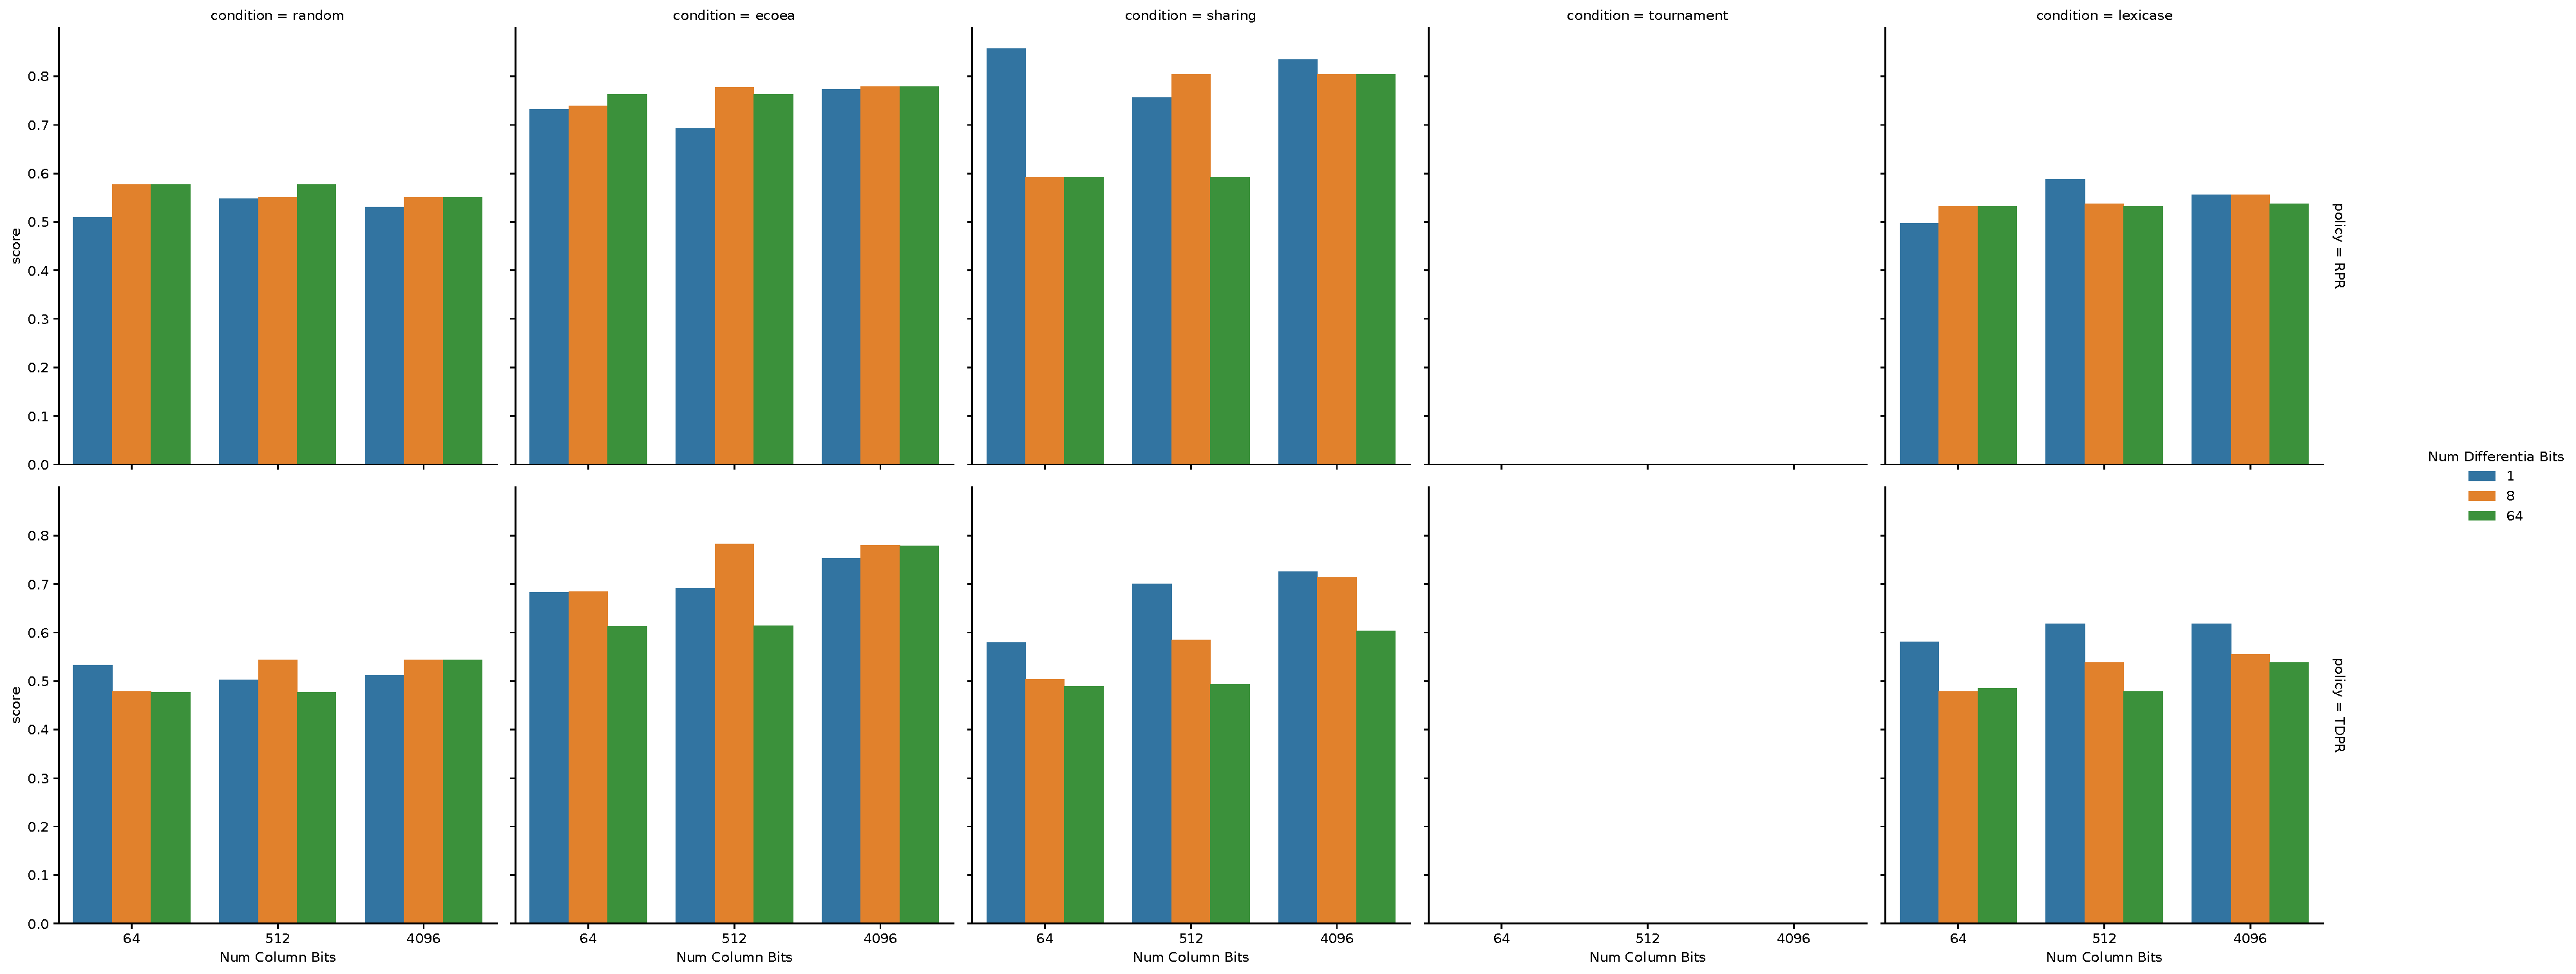
\includegraphics[width=\linewidth]{submodules/hereditary-stratigraph-concept/binder/reconstruction-quality/teeplots/col=condition+hue=num-differentia-bits+kind=bar+row=policy+tree-comparison-metric=mutual-clustering-information+viz=catplot+x=num-column-bits+y=score+ext=}
  \caption{
  Comparison of phylogenetic reconstruction quality across differentia bit counts.
  Reconstruction quality measured as mutual clustering information between reconstructed phylogeny and ground truth phylogeny \citep{smith2020information, smith2020treedist}.
  Higher is better.
  RPR is recency-proportional resolution stratum retention policy and TDPR is tapered depth-proportional resolution stratum retention policy.
  }
  \label{fig:diffbits-mutual-clustering-information}
\end{sidewaysfigure}
